
\chapter{Classification}

The project overview is show in Figure \ref{fig:cv-classification}:
\begin{figure}[!ht]
  \centering
  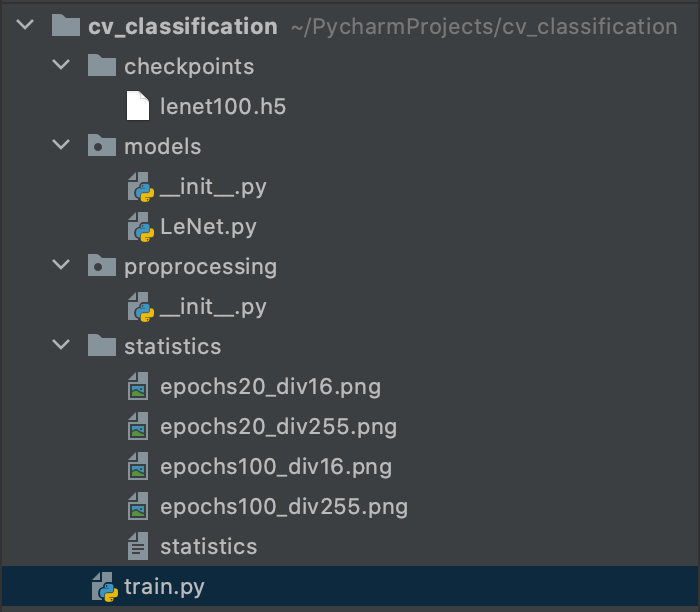
\includegraphics[width=\textwidth]{pics/cv-classification}
  \caption[CV Classification]{Compute Version Classification Project Overview}
  \label{fig:cv-classification}
\end{figure}



\section{train.py}

\begin{lstlisting}
#!/usr/bin/env python3
"""
@project: cv_classification
@file: train
@author: mike
@time: 2021/3/3
 
@function:
"""
from sklearn import datasets
from sklearn.model_selection import train_test_split
from sklearn.preprocessing import LabelBinarizer
from keras.optimizers import SGD
from keras import backend as K
from models.LeNet import LeNet
from sklearn.metrics import classification_report
import matplotlib.pyplot as plt
import numpy as np

# Step 1: load the dataset
print('[INFO] loading MNIST...')
dataset = datasets.load_digits()
# data
# target
# frame
# feature_names
# target_names
# images
# DESCR
data = dataset.data
target = dataset.target

# Step 2: process
# Step 2-1: scale the input arrange
data = data / 16.0  # from [0-16] to [0-1]
target = target.astype('int')

# Step 2-2: change shape
if K.image_data_format() == "channels_first":
    data = data.reshape(data.shape[0], 1, 8, 8)
else:
    data = data.reshape(data.shape[0], 8, 8, 1)

# Step 2-3: train, test split (this is optional)
# If the train test is split before the loading,
# there is no more split
train_x, test_x, train_y, test_y = train_test_split(data, target, test_size=0.2, random_state=16)

# Step 2-4: convert the labels from integers to vectors
lb = LabelBinarizer()
train_y = lb.fit_transform(train_y)
test_y = lb.transform(test_y)

# Step 3: initialize the optimizer and model
print('[INFO] compiling model...')
opt = SGD(learning_rate=0.01)
model = LeNet(width=8, height=8, depth=1, classes=10)
model.compile(loss="categorical_crossentropy", optimizer=opt, metrics=['accuracy'])

# Step 4: train the model
print('[INFO] training network...')
epochs = 100
# fit method can only be used for small dataset, for large dataset use the fit_generate instead
H = model.fit(train_x, train_y, batch_size=128, epochs=epochs, verbose=2, validation_data=(test_x, test_y))

# Step 5: evaluate the network
print("[INFO] evaluating network...")
predictions = model.predict(test_x, batch_size=128)

# step 6: save the model
model.save('checkpoints/lenet100.h5')

# Step 7: plot the train process
plt.style.use('ggplot')
plt.figure()
plt.plot(np.arange(0, epochs), H.history['loss'], label='train_loss')
plt.plot(np.arange(0, epochs), H.history['val_loss'], label='val_loss')
plt.plot(np.arange(0, epochs), H.history["accuracy"], label="train_acc")
plt.plot(np.arange(0, epochs), H.history["val_accuracy"], label="val_acc")
plt.title("Training Loss and Accuracy")
plt.xlabel("Epoch #")
plt.ylabel("Loss/Accuracy")
plt.legend()
plt.show()

# Step 8: write the statistics to a file (or just print)
statistics = classification_report(test_y.argmax(axis=1),
                                   predictions.argmax(axis=1),
                                   target_names=[str(x) for x in lb.classes_])
with open('statistics/statistics', 'w') as fh:
    for line in statistics:
        fh.write(line)  
\end{lstlisting}


\section{models/LeNet.py}

\begin{lstlisting}
#!/usr/bin/env python3
"""
@project: cv_classification
@file: LeNet
@author: mike
@time: 2021/3/3
 
@function:
"""
from keras.models import Sequential
from keras import backend as K
from keras.layers.convolutional import Conv2D, MaxPooling2D
from keras.layers.core import Activation, Flatten, Dense


def LeNet(width, height, depth, classes):
    model = Sequential()
    input_shape = (height, width, depth)

    if K.image_data_format() == 'channels_first':
        input_shape = (depth, height, width)

    model.add(Conv2D(20, (3, 3), padding='same', input_shape=input_shape))
    model.add(Activation('relu'))
    model.add(MaxPooling2D(pool_size=(2, 2), strides=(2, 2)))

    model.add(Conv2D(50, (3, 3), padding='same'))
    model.add(Activation('relu'))
    model.add(MaxPooling2D(pool_size=(2, 2), strides=(2, 2)))

    model.add(Flatten())

    model.add(Dense(500))
    model.add(Activation('relu'))

    model.add(Dense(classes))
    model.add(Activation('softmax'))

    return model
  
\end{lstlisting}


\section{Error and Anylysis}

At first, the division value used is 255.0 (train.py line 35).
Normally, this should make sense, becuase the value of image points lay in [0,255].
The output is as shown in Figure \ref{fig:div255-epochs20} (epochs=20) and \ref{fig:div255-epochs100} (epochs=100).
\begin{figure}[!ht]
  \centering
  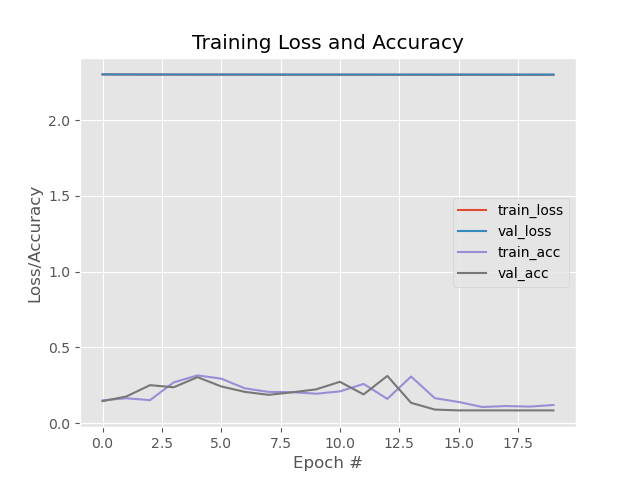
\includegraphics[width=\textwidth]{pics/epochs20_div255}
  \caption{Divide 255 and epochs=20}
  \label{fig:div255-epochs20}
\end{figure}


\begin{figure}[!ht]
  \centering
  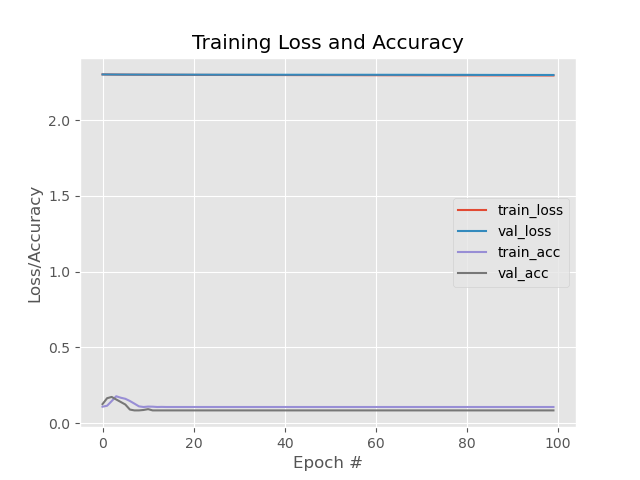
\includegraphics[width=\textwidth]{pics/epochs100_div255}
  \caption{Divide 255 and epochs=100}
  \label{fig:div255-epochs100}
\end{figure}


After diving into the dataset, I found that the maximum value is 16.
After changing the division to 16, the result is shown in Figure \ref{fig:div16-epochs20}.

\begin{figure}[!ht]
  \centering
  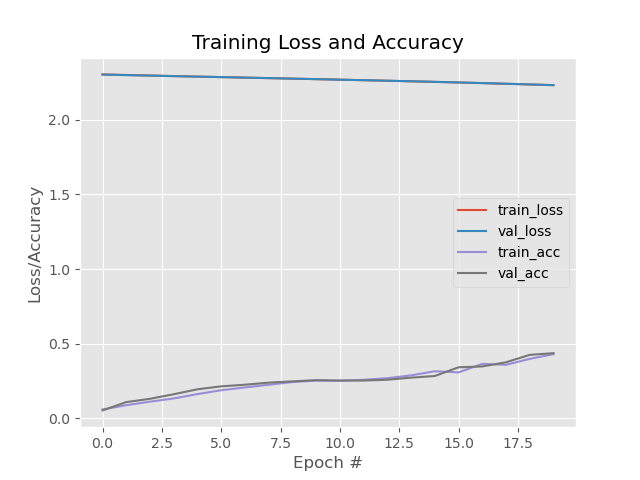
\includegraphics[width=\textwidth]{pics/epochs20_div16}
  \caption{Divide 16 and epochs=20}
  \label{fig:div16-epochs20}
\end{figure}


From the Figue \ref{fig:div16-epochs20} we can see that the epochs is too small.
After chaning the epochs to 100, the result is shown inf Figure \ref{fig:div16-epochs100}.
\begin{figure}[!ht]
  \centering
  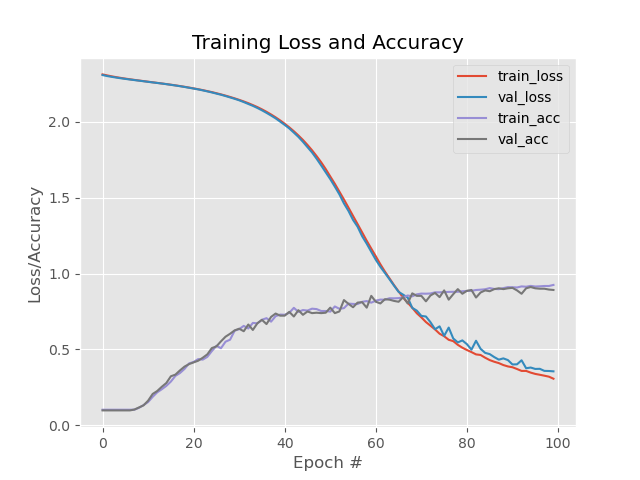
\includegraphics[width=\textwidth]{pics/epochs100_div16}
  \caption{Divide 16 and epochs=100}
  \label{fig:div16-epochs100}
\end{figure}